%
%  RULES OF THE GAME
%
%  * 80 characters
%  * line breaks at the ends of sentences
%  * eqnarrys ONLY
%  * ALWAYS cite inside parens () and use \citealt{}; no in-line cites
%  * that is all.
%

\documentclass[12pt,preprint]{aastex}

\include{vc}

\usepackage{color,hyperref}
\definecolor{linkcolor}{rgb}{0,0,0.5}
\hypersetup{colorlinks=true,linkcolor=linkcolor,citecolor=linkcolor,
            filecolor=linkcolor,urlcolor=linkcolor}
\usepackage{url}
\usepackage{amssymb,amsmath}
\usepackage{subfigure}

\newcommand{\project}[1]{{\sffamily #1}}
\newcommand{\emcee}{\project{emcee}}
\newcommand{\kepler}{\project{Kepler}}
\newcommand{\license}{MIT License}

\newcommand{\paper}{\emph{Article}}

\newcommand{\foreign}[1]{\emph{#1}}
\newcommand{\etal}{\foreign{et\,al.}}
\newcommand{\etc}{\foreign{etc.}}

\newcommand{\Fig}[1]{Figure~\ref{fig:#1}}
\newcommand{\fig}[1]{\Fig{#1}}
\newcommand{\figlabel}[1]{\label{fig:#1}}
\newcommand{\Tab}[1]{Table~\ref{tab:#1}}
\newcommand{\tab}[1]{\Tab{#1}}
\newcommand{\tablabel}[1]{\label{tab:#1}}
\newcommand{\Eq}[1]{Equation~(\ref{eq:#1})}
\newcommand{\eq}[1]{\Eq{#1}}
\newcommand{\eqlabel}[1]{\label{eq:#1}}
\newcommand{\Sect}[1]{Section~\ref{sect:#1}}
\newcommand{\sect}[1]{\Sect{#1}}
\newcommand{\App}[1]{Appendix~\ref{sect:#1}}
\newcommand{\app}[1]{\App{#1}}
\newcommand{\sectlabel}[1]{\label{sect:#1}}

\newcommand{\dd}{\ensuremath{\,\mathrm{d}}}
\newcommand{\bvec}[1]{\ensuremath{\boldsymbol{#1}}}
\newcommand{\appropto}{\mathrel{\vcenter{
  \offinterlineskip\halign{\hfil$##$\cr
    \propto\cr\noalign{\kern2pt}\sim\cr\noalign{\kern-2pt}}}}}

% TO DOS
\newcommand{\todo}[3]{{\color{#2} \emph{#1} TODO: #3}}
\newcommand{\dfmtodo}[1]{\todo{DFM}{red}{#1}}
\newcommand{\hoggtodo}[1]{\todo{HOGG}{blue}{#1}}
\newcommand{\mortontodo}[1]{\todo{MORTON}{green}{#1}}

% Document specific variables.
\newcommand{\rate}{\ensuremath{\eta}}
\newcommand{\ratepars}{{\ensuremath{\bvec{\theta}}}}
\newcommand{\obs}[1]{\ensuremath{\hat{#1}}}
\newcommand{\radius}{\ensuremath{R}}
\newcommand{\period}{\ensuremath{T}}
\newcommand{\completeness}{{\ensuremath{P_\mathrm{c}}}}
\newcommand{\transitprob}{{\ensuremath{P_\mathrm{t}}}}
\newcommand{\entry}{\ensuremath{S}}
\newcommand{\catalog}{{\ensuremath{\bvec{\entry}}}}
\newcommand{\binheight}{{\ensuremath{w}}}
\newcommand{\binheights}{{\ensuremath{\bvec{\binheight}}}}

\newcommand{\smoothreg}{{\ensuremath{\lambda}}}
\newcommand{\interim}{{\ensuremath{\bvec{\alpha}}}}

\begin{document}

\title{%
  Inferring the distribution and rate of Earth-like exoplanets \\
  from noisy individual-planet inferences
}

\newcommand{\nyu}{2}
\newcommand{\mpia}{3}
\newcommand{\princeton}{4}
\newcommand{\berkeley}{5}
\author{%
    Daniel~Foreman-Mackey\altaffilmark{1,\nyu},
    David~W.~Hogg\altaffilmark{\nyu,\mpia},
    Timothy~D.~Morton\altaffilmark{\princeton},
    Erik~A.~Petigura\altaffilmark{\berkeley},
    \etal
}
\altaffiltext{1}         {To whom correspondence should be addressed:
                          \url{danfm@nyu.edu}}
\altaffiltext{\nyu}      {Center for Cosmology and Particle Physics,
                          Department of Physics, New York University,
                          4 Washington Place, New York, NY, 10003, USA}
\altaffiltext{\mpia}     {Max-Planck-Institut f\"ur Astronomie,
                          K\"onigstuhl 17, D-69117 Heidelberg, Germany}
\altaffiltext{\princeton}{Department of Astrophysics, Princeton University,
                          Princeton, NJ, 08540, USA} % CHECK THIS ZIP CODE
\altaffiltext{\berkeley} {Department of Astronomy,
                          University of California at Berkeley,
                          Berkeley, CA, XXXXX, USA} % CHECK THIS ZIP CODE

\begin{abstract}
Although no true extra-solar Earth analog is known, hundreds of planets have
been found around Sun-like stars that are either Earth-sized but on shorter
periods, or else on year-long orbits but somewhat bigger than Earth.
These populations ought to permit a (possibly highly uncertain) extrapolated
measurement of the probability or rate at which Sun-like stars host true Earth
analogs.
Here we present a general probabilistic framework for making justified
inferences about the occurrence rate of exoplanets taking into account survey
completeness \emph{and observational uncertainties}.
We demonstrate that our method produces lower variance estimates than the
standard inverse-detection-efficiency weighting procedure.
When applied to an existing catalog of small planet candidates around G dwarfs
(Petigura \etal 2013), our method confirms previous measurements of a
flattening radius distribution near Earth's radius.
One output of our models is fully marginalized estimates---marginalizing out
observational uncertainties and all distribution parameters---of the rate
density of true Earth analogs, expressed as a number of planets per star per
natural logarithmic interval of period and radius, evaluated at the properties
of Earth.
The rate density we infer is an extrapolation; it depends strongly on the
permitted flexibility of the distribution model, but it tends to come out
at around ten percent, with large uncertainty.
\end{abstract}

\keywords{%
exoplanets: sickness
---
exoplanets: eta-Earth
---
code: open-source
---
keywords: made-up-by-Hogg
}

\section{Introduction}

\hoggtodo{%
\kepler\ has been busting out exoplanets (CITE).
Many of them even appear possibly rocky and habitable (CITE).
Nonetheless, none yet known are true Earth analogs.
}

\hoggtodo{%
This hasn't stopped anyone from estimating the rate at which Sun-like stars
host Earth-like planets on year-ish period orbits (CITE).
All of these rate estimates are extrapolations of one kind or another.
Here we perform an extremely conservative extrapolation of this kind.
}

\hoggtodo{%
What would make an extrapolation like this conservative?
Using \emph{huge bins} does not a conservative estimate make.
You don't want to assume separabilities you can't justify.
You want to explore an enormous function space for the exoplanet rates or pdf.
We are going to do be conservative in these senses here, far more conservative
than anyone who has come before.
}

This study is novel in a number of ways.
We create probabilistic information about the full exoplanet population
\emph{not} by weighting the detected objects by the inverse detection
efficiency (\citealt{petigura}), but rather by forward modeling the
observed distribution subject to the detection efficiency
(\dfmtodo{CITE TREMAINE?} \citealt{dong}).
Re-weighting the data by inverse selection probability---a method called
V-max in the quasar and galaxy luminosity function contexts---is not wrong,
but it produces a higher-variance estimate of the population than a justified
likelihood approach; it is higher variance because
the effective number of samples, after
weighting, can be much smaller than the actual number of samples.
In this work, we build a justified
likelihood of the observed data, taking into account the completeness function
or detection efficiency.
Our likelihood function is a variable-rate Poisson likelihood; it makes the
fundamental assumption that the data points are independently drawn from the
model, but is agnostic about all other properties of the data or distribution
functions.
Indeed, the assumptions behind this study here are weaker than those of any
previous study of the period and radius distribution of the Earth-sized
exoplanet population (\dfmtodo{CITE TREMAINE?} \citealt{dong, petigura}).

Another new aspect of this study is that it makes use of very flexible
distribution function models.
Indeed most of the models we consider are ``non-parametric'' in the weak sense
that they have enormous numbers of free parameters (not the strong sense of
having an \emph{infinite} number of free parameters).
The models are protected from degeneracies and over-fitting by priors.
In some models we assume that the two-dimensional distribution of planets in
period and radius is separable; in others we don't.
We treat all of these parameters as ``nuisance parameters'' when we ask
questions about the occurrence of Earth analogs.
That is, our rate conclusions are fully marginalized, and those
marginalizations are over non-trivial numbers of parameters.

When, in what follows, we ask questions about the radius disribution of
exoplanets, the distribution parameters are no longer nuisances The
radius-distribution parameters are what we are trying to measure.
Even in this case, however, our results will have the period-distribution
parameters marginalized out.

Perhaps the most important novelty of this study is in its treatment of
observational uncertainties.
Although planet periods in our data set are very precisely measured, the
planet radius measurements have large uncertainties.
The justified probabilistic approach to including these uncertainties in a
distribution analysis is to introduce the ``true'' radii as latent variables
and infer and marginalize them out along with all other nuisance parameters.
Although this sounds expensive---and it can be---there is a simple approach
we have been advocating (\cite{hogge}) that makes use of importance sampling.
We use this approach here; our results are fully marginalized over posterior
uncertainties in all of the planet radii.
More will be said about this below; the importance sampling looks like a
product over data points of sums (averages) over individual-datum radius
samplings.

\section{Model generalities}

\emph{Note: I think that we should use $T$ instead of $P$ for period because
$P$ is too heavily overloaded by the probabilities\ldots}

From our perspective, a ``model'' is a likelihood function---a probability
density (or distribution) function (PDF) for the data given
parameters---and a set of prior PDFs for the parameters.
In what follows, we will treat as ``data'' a catalog of exoplanet period
and radius measurements (\citealt{petigura}).
\emph{(I don't think need this next sentence).}
We will treat the uncertainties on those measurements as ``prior
information''; that is, we will treat those as true as given and not as being
generated by the parameterized likelihood function.

In the models that follow, the most important parameters will be parameters
of the PDF for the exoplanet periods and radii.
However, there will also be ``latent parameters'' that represent the ``true''
values of the exoplanet periods \period\ and radii \radius.
That is, for each exoplanet, there is a ``measured'' or ``observed'' period
\obs{\period}\ and radius \obs{\radius}, which constitute our data.
These relate to the unobserved ``true'' period and radius by a noise model.
For the conclusions of this study, the true values of period and radius are
nuisance parameters; we will marginalize them out.

Let's also introduce more succinct notation for a \emph{catalog}.
We'll refer to the set of period and radius measurements for a set of $K$
candidate exoplanets as
\begin{eqnarray}
\catalog &=& \{\entry_k\}_{k=1}^K
\end{eqnarray}
where each entry $\entry_k = (\period_k,\,\radius_k)$ is a tuple containing a
period and radius.

The purpose of this \paper\ is to determine constraints on the \emph{rate
function} of exoplanets
\begin{eqnarray}\eqlabel{true-rate}
\rate_\ratepars (\entry)
&=& \frac{\dd N}{\dd\ln\period\dd\ln\radius}
\end{eqnarray}
given our dataset.
Here we have not made any assumptions about the functional form of \rate, we
are only stating that it can be modeled by some---possibly very large---set of
parameters \ratepars.

In this \paper, we will assume that the completeness function of the survey is
known and it can be represented as a probability at every (true) period and
radius $\completeness (\entry)$.
This probability will also include the geometric transit probability as a
function of period $\transitprob (\period)$.
These selection effects can be incorporated into the rate from \eq{true-rate}
to get the \emph{observable rate}
\begin{eqnarray}\eqlabel{obs-rate}
\obs{\rate}_\ratepars (\entry)
&=& \rate_\ratepars(\entry)\,\completeness(\entry)\quad.
\end{eqnarray}

Given this parameterized rate $\obs{\rate}_\ratepars$, we can compute the
Poisson likelihood of a \catalog\ (\citealt{tabachnik,youdin,dong})
\begin{eqnarray}\eqlabel{true-like}
\ln p(\catalog\,|\,\ratepars) &\propto&
\sum_{k=1}^K \ln\obs{\rate}_\ratepars (\entry_k)
- \int \obs{\rate}_\ratepars (\entry) \dd\entry
\end{eqnarray}
where we have assumed that every object in \catalog\ is an independent
Poisson sample from the rate.

If we had perfect noiseless measurements of the periods and radii for every
object in our catalog, \eq{true-like} provides a metric for determining
constraints on the parameters of the rate function.
In practice, the measurements of \catalog\ are noisy so we need to include
these effects.

\section{Including observational uncertainties}

The likelihood function given in \eq{true-like} is a model of the
probability of observing a catalog with \emph{true} periods and radii.
If we want to include the effects of measurement uncertainties, we need to
take a moment to consider the meaning of measurement uncertainties.

The catalog of planet candidates considered in this \paper\
(\citealt{petigura}) was generated by drawing samples from a posterior
probability distribution for physical parameters (period, radius, impact
parameter, \etc) conditioned on \kepler\ light curves.
The $k$th entry in this catalog is, therefore, a representation of the
posterior PDF
\begin{eqnarray}\eqlabel{measurement}
p(\entry_k\,|\,\obs{\entry}_k,\,\interim)
\end{eqnarray}
using the notation from the previous section.
In \eq{measurement}, the notations \interim\ indicates that the measurement
was made with a specific choice of prior over parameters
$p(\entry_k\,|\,\interim)$.
We will refer to these priors as \emph{interim priors} because our goal is to
infer the distribution that is consistent with the data.

More generally, a published catalog represents a \emph{posterior PDF over
plausible catalogs}
\begin{eqnarray}\eqlabel{catalog-pdf}
p(\catalog\,|\,\obs{\catalog},\,\interim) \quad.
\end{eqnarray}
It is normally safe to assume that each entry in the catalog is conditionally
independent given the choices of interim priors.
\dfmtodo{Why and when is this a good/bad/necessary assumption?}
Under this assumption, \eq{catalog-pdf} factorizes as
\begin{eqnarray}\eqlabel{catalog-factor}
p(\catalog\,|\,\obs{\catalog},\,\interim) &=&
\prod_{k=1}^K p(\entry_k\,|\,\obs{\entry}_k,\,\interim) \quad.
\end{eqnarray}

It will be useful in the following discussion to represent the catalog PDF as
a set of $N$ samples
\begin{eqnarray}\eqlabel{catalog-samples}
\catalog^{(n)} &\sim& p(\catalog\,|\,\obs{\catalog},\,\interim) \quad.
\end{eqnarray}
For the general catalog, these could be generated using MCMC or a similar
sampling algorithm.
Under the conditional independence assumption of \eq{catalog-factor}, however,
the problem is much simpler.
Each entry $\entry_k$ can be sampled independently and then the catalog
samples $\catalog^{(n)}$ are given by the outer product of the independent
sample lists.

Now that we have a representation of the catalog, we want to infer constraints
on the occurrence rate of exoplanets conditioned on all the data.
To perform this inference, we need to compute the  \emph{marginalized
likelihood}
\begin{eqnarray}\eqlabel{marg-likelihood}
p(\obs{\catalog}\,|\,\ratepars) &=&
\int p(\catalog,\,\obs{\catalog}\,|\,\ratepars) \dd\catalog \quad.
\end{eqnarray}
The marginalized likelihood measures the probability of all the \kepler\ light
curves given a particular setting of the occurrence rate parameters.
If we can efficiently compute this then we can optimize to find the
maximum likelihood occurrence rate or we can apply priors $p(\ratepars)$ and
sample to find posterior constraints on the occurrence rate.
Note that any results obtained through \eq{marg-likelihood} will
\emph{correctly account for all the measurement uncertainties}.

The integral in \eq{marg-likelihood} cannot be computed analytically and, in
fact, it will generally be extremely computationally expensive to evaluate
numerically (\dfmtodo{CITE}).
In our case, however, we only need to evaluate this integral up to a constant
and there is a simple approximation---using the sampling representation of the
catalog---that can be sufficiently accurate for our purposes.
To derive this approximation, first recall that the joint distribution inside
the integral in \eq{marg-likelihood} factorizes as
\begin{eqnarray}
p(\catalog,\,\obs{\catalog}\,|\,\ratepars) &=&
p(\catalog\,|\,\ratepars)\,p(\obs{\catalog}\,|\,\catalog)
\end{eqnarray}
because the occurrence rate generates the \emph{true} distribution of periods
and radii.
Then, we can multiply the integrand by
\begin{eqnarray}
\frac{p(\catalog\,|\,\obs{\catalog},\,\interim)}
     {p(\catalog\,|\,\obs{\catalog},\,\interim)}
\end{eqnarray}
and simplify to find
\begin{eqnarray}
\frac{p(\obs{\catalog}\,|\,\ratepars)}
     {p(\obs{\catalog}\,|\,\interim)}
&=&
\int \frac{p(\catalog\,|\,\ratepars)}{p(\catalog\,|\,\interim)}\,
p(\catalog\,|\,\obs{\catalog},\,\interim)
\dd\catalog \quad.
\end{eqnarray}
Using the samples over catalogs $\catalog^{(n)}$ as defined above, we can
approximate this integral---up to an irrelevant normalization constant---as
\begin{eqnarray}\eqlabel{approx-marg-likelihood}
p(\obs{\catalog}\,|\,\ratepars) &\appropto&
\sum_{n=1}^N
\frac{p(\catalog^{(n)}\,|\,\ratepars)}{p(\catalog^{(n)}\,|\,\interim)}
\end{eqnarray}
where the numerator inside the sum is given by \eq{true-like} and the
denominator is the interim prior evaluated at the coordinates of the samples.

This is a generalization of the approximation presented previously in the
exoplanet literature (\citealt{hogge}) but in this case, the likelihood
function \eq{true-like} doesn't factorize over entries in the catalog.
As a result, the variance of \eq{approx-marg-likelihood} is more sensitive to
the choice of interim prior.
In practice, we have found that including the completeness function
$\completeness(\entry)$ in $p(\entry\,|\,\interim)$ greatly improves
performance.
This term can be incorporated into existing samplings---generated using less
informative priors---using rejection sampling.

\section{Parameterization of the occurrence rate}

In the following sections, we will model the occurrence rate
$\rate(\period,\,\radius)$ as a two dimensional grid with $N_\period$ bins in
$\ln\period$ and $N_\radius$ bins in $\ln\radius$.
We choose to fix the bin locations leaving only the bin heights
$\binheights = \{\binheight_{ij}\}_{i=1,j=1}^{N_\period,N_\radius}$ as
free parameters.
In practice, the results seem to be more numerically stable---but the model is
exactly equivalent---when we model the rate as
\begin{eqnarray}
\rate(\period,\,\radius) &=& \rate_0\,p(\period,\,\radius)
\end{eqnarray}
where $\rate_0$ is the total rate of planets in the sample and the relative
probability factor is subject to the constraint
\begin{eqnarray}
1 &=& \int p(\period,\,\radius) \dd\period\dd\radius\quad.
\end{eqnarray}
In this model, the parameter set \ratepars\ includes $\rate_0$ and the heights
of all but one of the bins in $p(\period,\,\radius)$.

Since the choice of bin locations and number is arbitrary, the most
conservative strategy is to choose very small bins---yielding an effectively
non-parametric model---and choose a prior (or regularization) that encodes any
prior expectations about the distribution.
In particular, it seems reasonable to expect the distribution to be
``smooth''.
The most extreme version of this model would be a completely non-parametric
rate function---generated by, for example, a Gaussian process
(\citealt{poiss-gp})---but this discussion is beyond the scope of this
\paper.
Instead, we'll simply choose small bins and add a term to the likelihood
function that penalizes large changes between neighboring bins.
Specifically, we choose a term of the form
\begin{eqnarray}
\ln p(\binheights\,|\,\smoothreg_\period,\,\smoothreg_\radius) &=&
-\frac{1}{2}\sum_{i=2}^{N_\period}
\frac{|\binheights_{i,\cdot} - \binheights_{i-1,\cdot}|^2}{\smoothreg_\period}
-\frac{1}{2}\sum_{j=2}^{N_\radius}
\frac{|\binheights_{\cdot,j} - \binheights_{\cdot,j-1}|^2}{\smoothreg_\radius}
-\frac{1}{2}\ln (\smoothreg_\period\,\smoothreg_\radius)
\quad.
\end{eqnarray}
In our final analysis, we'll marginalize over the regularization strengths
$\smoothreg_\period$ and $\smoothreg_\radius$ but we'll also explore the
effects of this choice below.

\section{The completeness function \& dataset}

\dfmtodo{%
Describe Erik's data products and our model of the completeness in boxes
extended artificially beyond the original range.
Also describe the re-sampling procedure for the candidate parameters.
}

\section{Synthetic catalogs}

The likelihood function in \eq{true-like} provides a \emph{probability
distribution over catalogs} conditioned on the parameters of the rate
function.
Therefore, it is also the description of a \emph{generative process} for
synthetic catalogs.
To demonstrate the effectiveness of our model, we generate synthetic catalogs
from known distributions in period and radius, and test the performance of our
method on the resulting data.
For comparison, we also implement the one-over-efficiency weighting procedure
(see, for example, \citealt{howard, dressing, petigura}) and apply it to the
same datasets.

\paragraph{The generative process}
The variable rate Poisson likelihood function in \eq{true-like} can be sampled
generally for arbitrary forms of the rate function using a procedure called
``thinning'' (\citealt{poisson}).
In this \paper, however, we will only consider binned representations of
\rate, greatly simplifying the generative process.
Conditioned on a set of rate function parameters and a given completeness
function (here we'll use the injections from \citealt{petigura}), we compute
the observable rate grid from \eq{obs-rate}.
Then in each bin, we sample $J$ candidates uniformly in period and
radius (as defined by the bin edges) where $J$ is a Poisson random variable
sampled with the rate given by the observable rate in this bin.
\dfmtodo{Make this description not be the most confusing thing ever.}
Then, we add 30\% measurement uncertainties to the radius measurements where
30\% was chosen to match to properties of the real catalog
(\citealt{petigura}).

\paragraph{Results}
See \fig{synthetic-radius}.
As expected, the forward model is a much lower variance estimator.

\begin{figure}[htbp]
\begin{center}
\subfigure[one-over-efficiency]{%
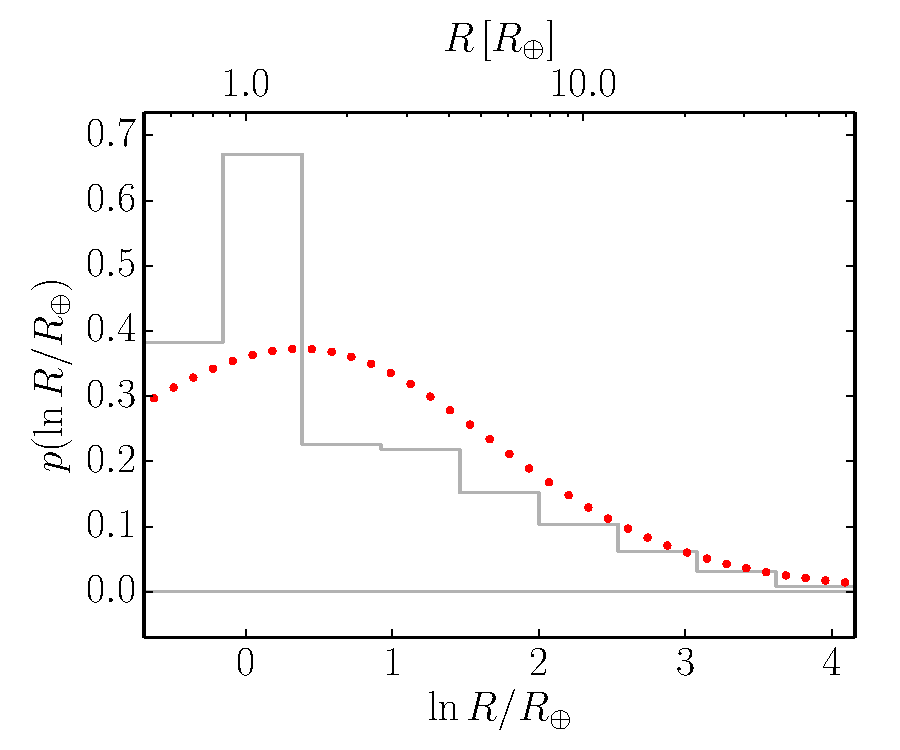
\includegraphics[width=0.45\textwidth]{figures/synthetic-vmax-radius.pdf}
}
\subfigure[fully-marginalized forward model]{%
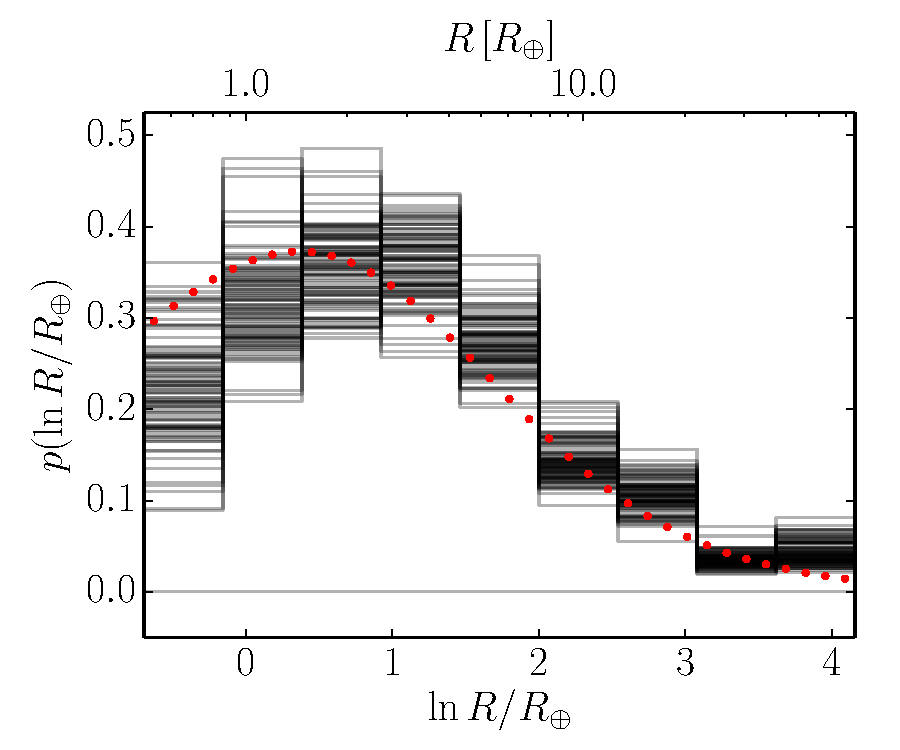
\includegraphics[width=0.45\textwidth]{figures/synthetic-radius.pdf}
}
\end{center}
\caption{%
The inferred distribution of exoplanet radii based on a noisy observation of a
synthetic catalog.
The red dotted line shows the true distribution function and the black
histograms are the constraints from the different inference techniques.
\figlabel{synthetic-radius}}
\end{figure}

\section{Real data}

It has been shown that the joint period--radius distribution for exoplanets is
not separable (\dfmtodo{CITE}).
In this section, we discuss non-separable model in our analysis framework.

We model the rate function $\rate(\period,\,\radius)$ as a piecewise constant
function in rectangular bins in $\ln\period$ and $\ln\radius$.
The parameters \ratepars\ that we're fitting are the values of each of these
bins (subject to a normalization constraint).

\section{Discussion}

We have made the first measurement of the Earth-like exoplanet population that
is based on forward modeling, takes proper account of the observational
uncertainties on planet radii, and makes use of extremely flexible
non-separable distributions for period and radius.
We find \hoggtodo{BLAH BLAH BLAH.}

Although our method makes weaker assumptions than any previous work in this
area, of course it \emph{does} make strong assumptions.
It assumes that the data set (from \citealt{petigura}) contains planets and
only planets (no false positives).
It assumes that the individual-planet radius uncertainties are also correctly
determined.
It assumes that the completeness calculation (again from \citealt{petigura})
is accurate and smoothly varying with period and radius; it makes no attempt
to adjust the completeness star-by-star for brightness or variability.
It assumes that the exoplanets are all independently drawn from the same
distribution function, with no regard to age, metallicity, or multiplicity.

Although we have taken account of the radius uncertainties in a principled
way, we did make one important approximation: We ignored planets with central
values far outside the period and radius box in which we built the model.
That is, we assumed that there are no very large outliers in radius
determination.
This assumption is a complex one; it involves the effective, end-to-end error
distribution in the data set, but also smoothness of the distribution function
at or near the edges of the analysis box.

If our inferences are right about true Earth analogs, then we expect that
there are about XXX transiting Earth analogs hidden in the \kepler\ data set.
We would be able to find some of these Earth analogs if the effective noise
level in the data could be reduced by a factor of about XXX.
We have identified a number of directions along which this noise reduction
might happen, including but not limited to retrospective data-driven or
physics-driven recalibrations of the \kepler\ focal plane
(\citealt{hoggwhitepaper}), new methods for performing aperture photometry,
and better models for stochastic instrument variability or stochastic
intrinsic stellar variability that take account of frequency structure
(\citealt{brewer, carter, roberts}).
If any (or all) of these deliver substantial improvements for \kepler\
archival data reanalyses, it's Nobel Prize time!  (Or at least \textsl{The
Colbert Report}?)

All of the code used in this project is available from
\url{http://github.com/dfm/exopop} under the MIT open-source software license.
This code (plus some dependencies) can be run to re-generate all of the
figures and results in this \paper; this version of the paper was generated
with git commit \texttt{\githash} (\gitdate).

\acknowledgments
It is a pleasure to thank
    \ldots
for helpful contributions to the ideas and code presented here.
This project was partially supported by the NSF (grant AST-0908357), and NASA
(grant NNX08AJ48G).
This research made use of the NASA \project{Astrophysics Data System}.

\newcommand{\arxiv}[1]{\href{http://arxiv.org/abs/#1}{arXiv:#1}}
\begin{thebibliography}{}\raggedright

\bibitem[Adams, Murray \& MacKay(2009)]{poiss-gp}
Adams, R.~P., Murray, I., \& MacKay, D.~J.~C.\ 2009, ICML, 2009, 9
(\href{http://homepages.inf.ed.ac.uk/imurray2/pub/09poisson/}{online})

\bibitem[Brewer \& Stello(2009)]{brewer}
Brewer, B.~J., \& Stello, D.\ 2009, \mnras, 395, 2226 (\arxiv{0902.3907})

\bibitem[Carter \& Winn(2009)]{carter}
Carter, J.~A., \& Winn, J.~N.\ 2009, \apj, 704, 51 (\arxiv{0909.0747})

\bibitem[Dong \& Zhu(2013)]{dong}
Dong, S., \& Zhu, Z.\ 2013, \apj, 778, 53 (\arxiv{1212.4853})

\bibitem[Dressing  \& Charbonneau(2013)]{dressing}
Dressing, C.~D., \& Charbonneau, D.\ 2013, \apj, 767, 95 (\arxiv{1302.1647})

\bibitem[Hogg \etal(2013)]{hoggwhitepaper}
Hogg, D.~W., Angus, R., Barclay, T., et al.\ 2013, \arxiv{1309.0653}

\bibitem[Hogg \etal(2010)]{hogge}
Hogg, D.~W., Myers, A.~D., \& Bovy, J.\ 2010, \apj, 725, 2166
(\arxiv{1008.4146})

\bibitem[Howard \etal(2012)]{howard}
Howard, A.~W., Marcy, G.~W., Bryson, S.~T., et al.\ 2012, \apjs, 201, 15
(\arxiv{1103.2541})

\bibitem[Lewis \& Shedler(1979)]{poisson}
Lewis, P.~A.~W., \& Shedler, G.~S.\ 1979, Naval Research Logistics Quarterly,
26, 403

\bibitem[Petigura \etal(2013a)]{petigura-a}
Petigura, E.~A., Marcy, G.~W., \& Howard, A.~W.\ 2013a, \apj, 770, 69
(\arxiv{1304.0460})

\bibitem[Petigura \etal(2013b)]{petigura}
Petigura, E.~A., Howard, A.~W., \& Marcy, G.~W.\ 2013b,
Proceedings of the National Academy of Science, 110, 19273 (\arxiv{1311.6806})

\bibitem[Roberts \etal(2013)]{roberts}
Roberts, S., McQuillan, A., Reece, S., \& Aigrain, S.\ 2013, \mnras, 435, 3639
(\arxiv{1308.3644})

\bibitem[Tabachnik \& Tremaine(2002)]{tabachnik}
Tabachnik, S., \& Tremaine, S.\ 2002, \mnras, 335, 151
(\arxiv{astro-ph/0107482})

\bibitem[Youdin(2011)]{youdin}
Youdin, A.~N.\ 2011, \apj, 742, 38 (\arxiv{1105.1782})

\end{thebibliography}

\end{document}
